% !TEX TS-program = pdflatex
% !TEX encoding = UTF-8 Unicode

%\documentclass[12pt,a4paper]{memoir} % for a long document
\documentclass[12pt,a4paper,article]{memoir} % for a short document

\usepackage[utf8]{inputenc} % set input encoding to utf8

%%% PAGE DIMENSIONS
% Set up the paper to be as close as possible to both A4 & letter:
\settrimmedsize{11in}{210mm}{*} % letter = 11in tall; a4 = 210mm wide
\setlength{\trimtop}{0pt}
\setlength{\trimedge}{\stockwidth}
\addtolength{\trimedge}{-\paperwidth}
\settypeblocksize{*}{\lxvchars}{1.618} % we want to the text block to have golden proportionals
\setulmargins{50pt}{*}{*} % 50pt upper margins
\setlrmargins{*}{*}{1.618} % golden ratio again for left/right margins
\setheaderspaces{*}{*}{1.618}
\checkandfixthelayout 
\usepackage{enumitem}
\setitemize{noitemsep,topsep=0pt,parsep=0pt,partopsep=0pt}
\usepackage{xcolor,listings}
\usepackage{textcomp}
\lstset{upquote=true}
\usepackage{graphicx}
\usepackage{subcaption}
\usepackage{hyperref}
\hypersetup{
  colorlinks=true,
  linkcolor=blue,
  urlcolor=blue
}

%%% \maketitle CUSTOMISATION
% For more than trivial changes, you may as well do it yourself in a titlepage environment
\pretitle{\begin{center}\sffamily\huge\MakeUppercase}
\posttitle{\par\end{center}\vskip 0.5em}

%%% ToC (table of contents) APPEARANCE
\maxtocdepth{subsection} % include subsections
\renewcommand{\cftchapterpagefont}{}
\renewcommand{\cftchapterfont}{}     % no bold!

%%% HEADERS & FOOTERS
\pagestyle{ruled} % try also: empty , plain , headings , ruled , Ruled , companion

%%% CHAPTERS
\chapterstyle{hangnum} % try also: default , section , hangnum , companion , article, demo

\renewcommand{\chaptitlefont}{\Huge\sffamily\raggedright} % set sans serif chapter title font
\renewcommand{\chapnumfont}{\Huge\sffamily\raggedright} % set sans serif chapter number font

%%% SECTIONS
\hangsecnum % hang the section numbers into the margin to match \chapterstyle{hangnum}
\maxsecnumdepth{subsection} % number subsections

\setsecheadstyle{\Large\sffamily\raggedright} % set sans serif section font
\setsubsecheadstyle{\large\sffamily\raggedright} % set sans serif subsection font

\newlength\drop
\makeatletter
\newcommand*\titleM{\begingroup%
\setlength\drop{0.08\textheight}
\centering
\vspace*{\drop}
{\Huge\bfseries Technical Interview}\\[\baselineskip]
%{\scshape MAN-AHL}\\[\baselineskip]
\vfill

\includegraphics[width=0.6\textwidth]{img/logo.png}\par\vspace{1cm}
\vfill
{\Huge\scshape Fadil Mokhchane \\ 
\small \href{https://www.linkedin.com/in/fadil/}{CV on LinkedIn} }\par
\vspace{1cm}

\includegraphics[width=0.3\textwidth]{img/harrington.jpg}\par
\vfill
\vspace*{2\drop}
{\scshape September 3, 2017}\par
{\scshape \small Version 1.0}\par
\endgroup}
\makeatother
%% END Memoir customization

\title{Technical Interview}
\author{Fadil Mokhchane}
%\date{ August 2017} % Delete this line to display the current date
%%% BEGIN DOCUMENT
\begin{document}


\begin{titlingpage}
\titleM
\end{titlingpage}

\newpage
\tableofcontents* % the asterisk means that the contents itself isn't put into the ToC
%\clearpage %or \cleardoublepage
\phantomsection
\listoffigures
\listoftables
\vfill
\newpage

%-------------------------------------------------------------------------------
\chapter{Algorithm Exercise}
\section{Question}
Implement the method nextNum() and a minimal but effective set of unit tests. 
Implement in the language of your choice, Python is preferred, but Java and 
other languages are completely fine. 
Make sure your code is exemplary, as if it was going to be shipped as part of a production system.

As a quick check, given Random Numbers are $[-1, 0, 1, 2, 3]$ and 
Probabilities are $[0.01, 0.3, 0.58, 0.1, 0.01]$ if we call nextNum() 100 times 
we may get the following results. As the results are random, these particular results are unlikely.
\begin{itemize}
	\item -1: 1 times 
	\item 0: 22 times
	\item 1: 57 times 
	\item 2: 20 times
	\item 3: 0 times 
\end{itemize}

%-------------------------------------------------------------------------------
\section{The Problem}
\label{sec:problem}
We interpret the question as the following the mathematical problem. 
We define $X$ as a discrete random variable. 
As input, we have a $k$ values, $x_i$, with their associated probabilities, $p_i$.

A discrete probability density function is a probability distribution charaterised 
by a probability mass function, c.f. \autoref{eq:pdf}, referenced as PDF.
\begin{equation}
	\forall i \in \left[1 ...  k\right], P\left[ X = x_i \right] = p_i  
	\label{eq:pdf}
\end{equation}
With
\[ 
	\sum_{i = 1}^k  P\left[ X = x_i \right]  = 1
\]
The values $\left(x_i, p_i\right)$ are called the PDF pillars.
This probability mass function can be illustrated by \autoref{fig:distribution} :
\begin{figure}[h!]
\begin{center}
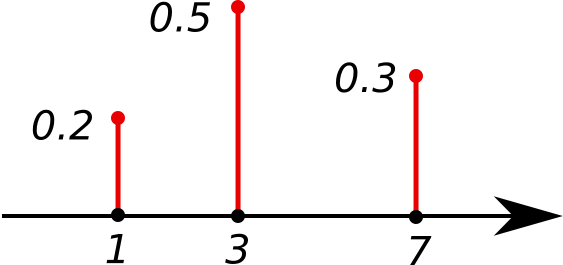
\includegraphics[width=0.5\textwidth]{img/distribution.png}
\caption{Probability Mass Function}
\label{fig:distribution}
\end{center}
\end{figure}

We would like to build a generator that picks $x_i$ given their probabilities
$P_i$. 
In order to make sure we generate $x_i$ with repesct to their original probabilities, 
we need to add a no $x_i$ selected if the sum of the $x_i$ is less than $1$.

This way we can build a discrete cumulative function, referenced as CDF,
 for $X$, $F_x$, such as :
\begin{equation}
	F_x = P\left( X \leq x \right)
	\label{eq:cdf}
\end{equation}
Which can be illustrated with \autoref{fig:cdf2} :
\begin{figure}[h!]
\begin{center}
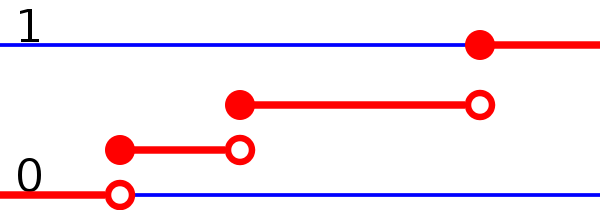
\includegraphics[width=0.5\textwidth]{img/cdf.png}
\caption{Discrete Cumulative Distribution Function}
\label{fig:cdf2}
\end{center}
\end{figure}

We then use a bounded uniform distribution, $U\left(0,1\right)$,
to generate random numbers between $0$ and $1$.
We picked two pseudo random numbers generator : Mersenne Twister\footnote{
The Mersenne twister is a pseudorandom number generator developed by 
Makoto Matsumoto and Takuji Nishimura that is based on a matrix linear 
recurrence over a finite binary field. 
It has a period of $2^{63}-1$.
The source for the C code can be found 
\href{http://www.math.sci.hiroshima-u.ac.jp/~m-mat/MT/emt64.html}{here}.
} (This implementation claims to be faster than Ecuyer's one.) and Ecuyer\footnote{
This is the default random number generator in haskell.
 This implementation uses the Portable Combined Generator of L'Ecuyer
 for 32-bit computers, transliterated in Haskell by Lennart Augustsson. 
 It has a period of roughly $2.30584e18$.
 } in order to compare and pick the best one.

Finally using the inverse of the discrete cumulative function, reference as Inverse CDF, 
we can pick an $x_i$, described in \autoref{eq:invcdf}.
\begin{equation}
	\forall y \in \left[0...1 \right], F^{-1}_y = x_i
	\label{eq:invcdf}
\end{equation}
This process gives us a weighted probability pseudo random number engine.

%-------------------------------------------------------------------------------
\section{Solution Proposed}
\subsection{Overview}

The key requirement is to deliver a production quality software.
This means that the code has to be well designed, simple, 
efficient, portable and well tested.

The key features we would like to achieve :
\begin{itemize}
	\item Implement the weighted probability engine\footnote{
		The task of an engine is to manage the creation of a serie of
		pseudo random numbers.} based
		on a bounded uniform random probability engine,
	\item Target a $100\%$ testing coverage.
	\item Assess the quality of our probability engines,
	\item Assess the performances of our probability engines,
	\item Create an User Interface, via Command Line Input,
	\item Document the work.
\end{itemize}

\subsection{Design}
We target the following archictecture, c.f. \autoref{fig:architecture1}.
\begin{figure}[h!]
\begin{center}
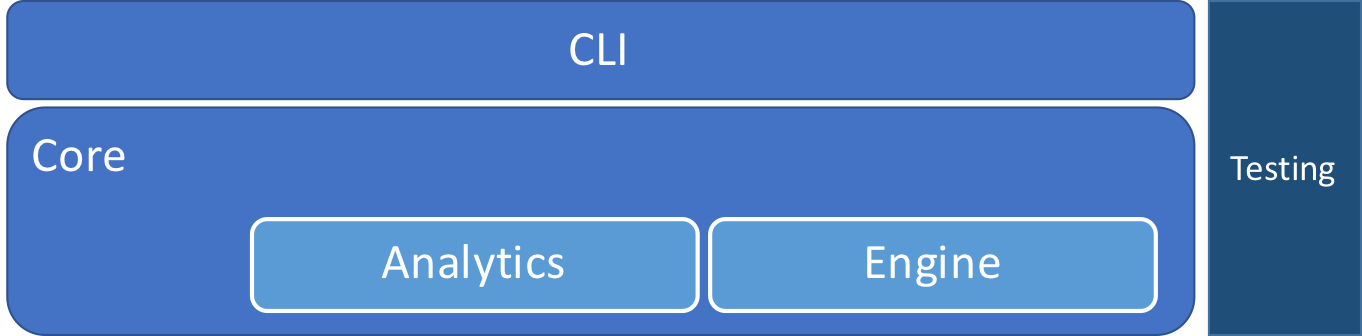
\includegraphics[width=0.8\textwidth]{img/architecture1.png}
\caption{Algorithm App Architecture}
\label{fig:architecture1}
\end{center}
\end{figure}
The various modules implement all the functionalities we need.
\begin{description}
	\item[Analytics] The mathematical functions required,
	
	In this module we have the implementation of the discrete 
	probability function\footnote{
	We can take as input incomplete probabilities, i.e. that
	don't sum up to $1$. We therefore assign the remaining
	probability to the event we don't select any element.
	Haskell provides the \emph{Maybe a} type to modelise this.
	}, the discrete cumulative function, 
	the inverse discrete cumulative function, the mean and
	standard deviation functions.
	
	\item[Uniform Engine] The bounded uniform 
	pseudo random numbers engine,
	
	This module contains an abstraction to a uniform pseudo
	random number generator with values bounded 
	within $ \left[ 0, 1 \right]$.
	It can compute a random number or a series of random 
	number and the statistics related to the distribution of 
	the random number generated.
	\item[Weighted Engine] 	The weighted pseudo random 
	numbers probability engine,
	
	This module includes an abstraction to the weighted 
	pseudo random numbers generators.
	It allows computation and statistics on these numbers.
	It includes the requested nextNum function.
	\item[CLI] 		The command line input layer,
	
	As it is meaningless to look only at one random number at the time.
	The CLI provides a flexible API to compute
	statistics on $n$ random numbers.
	We can select any random number engine we have implemented.
	We display only the distribution of these random numbers.
	\item[Testing] 	The testing module,
	
	This module provides all the automated tests. They are unit 
	tests at the module level and integration tests at the key
	features level.
\end{description}


\subsection{User Interface}
The UI is a command line input allowing the user to run each feature.
After building the project, with the following command:
\begin{verbatim}
cabal build
\end{verbatim}
The binary is then located in \emph{./dist/build/MAN-AHL/MAN-AHL}.
We can run the weighted or the uniform engine
 as described in \autoref{fig:cli}, with the following command:
\begin{verbatim}
time ./dist/build/MAN-AHL/MAN-AHL -run=Weighted -nSims=1000000
        -pillars='[(1, 0.5), (2, 0.5)]'
\end{verbatim}
 The binary has the option \emph{-help}, stating all the default values.
\begin{figure}[h!]
\begin{center}
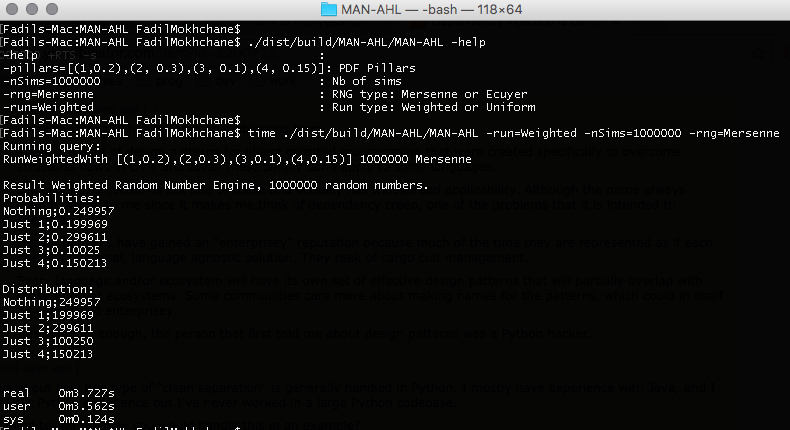
\includegraphics[width=1\textwidth]{img/cli.png}
\caption{Command Line Input}
\label{fig:cli}
\end{center}
\end{figure}

%-------------------------------------------------------------------------------
\section{Implementation}

We use Haskell as implementation language. It is a purely functional language.
It has a strong type system. It is all about types, they tell the story.
In this section, we introduce the key types used thoughout the application.

\subsection{General Notes}
We use efficient data structures as appropriate and we modelise the problem using
the whole power of Haskell. 
We use \emph{newtype} as much as possible as it allows design at a 
seemless cost.

Indeed, we use parametric and ad hoc polymorphism as needs be.
We modelise the exception handling using different techniques, depending on
the context, let it be \emph{Either a b}, \emph{Maybe a} or \emph{error}. 

The aim was to keep the software as simple as possible while targeting a
good design and performance. 

The code is documented while we believe that a simple and well organised
code needs less documentation. The complexities are presented in the some
area of the code. 

Any constructive feedback is most welcome.

\subsection{Analytics Module}

The analytics are mainly destined to weighted probability engine.

We define the \emph{PieceWiseCurve x y} algebraic data type(ADT) to provide an
abstraction to piecewise curve, as we are working with discrete
random variable, it is the closest to reality. We picked the tree map data
structure, \emph{Data.Map} in Haskell, to get efficient lookup ( O(log n) ).
The \emph{Curve x y a} class\footnote{ad hoc polymorphism} 
provides the key operations on a 
\emph{PieceWiseCurve}.  

We subsequently define the ADTs to represent all the curves we need
for our weighted probability engine :
\begin{itemize}
	\item The \emph{PDF} ADT modelising the probability mass function,
	The key are the $x_i$ and the values the $p_i$, we presented in
	\autoref{sec:problem}.
	We merge the pillars with similar $x_i$, discard the pillars with zero
	$p_i$ and ensure that $\sum_i p_i \leq 1$.
	If needed we add a pillar representing non selected element 
	as \emph{Nothing}. This way we ensure that the probabilities
	adds up to 1.
	\item The \emph{CDF} ADT represents the discrete cumulative
	curve, presented in \autoref{fig:cdf2}.
	\item The \emph{InvCDF} ADT represents the inverse CDF curve,
	as explained in \autoref{eq:invcdf}
	\item The \emph{Distribution a} ADT models a distribution curve
	of the random number generated.
\end{itemize}
Again, we refer to curve as to piecewise curves or histograms.

This module contains also the basic statistics we are using to 
analyse the results.

\subsection{Uniform Engine Module}

The \emph{UniformRNG} ADT abstracts a choice of uniform pseudo random 
number generator, Mersenne Twister and Ecuyer. We could seemlessly
add new generator, if needs be. We would need to extend the standard
Haskell \emph{RandomGen} class. 
They can generate un-bounded pseudo random numbers.

The \emph{ProbaUniEngine} ADT abstracts the computation of a uniform pseudo
random number generation bounded between 0 and 1.
It uses the \emph{State} monad to pass on the state of \emph{UniformRNG}
when we combine multiple computations.
This engine instanciates the \emph{ProbaEngine} class, which define
and abstract the role of a probability engine. The latter is to 
create one or a series of pseudo random numbers.

The \emph{StatUniEngine} ADT abstracts the computation of the statistics
related to the bounded uniform random numbers generated. 
In order to be efficient, we compute only the distribution while we 
are creating pseudo random numbers. 
There is a post-processing step at the end of the simulation, which 
computes the remaining relevant statistics.
It uses the \emph{State} monad to pass on the state of the 
uniform random number generator and the cumulative statistics.
This engine instanciates the \emph{StatEngine} class, which role is
to compute the statistics of a series of random numbers.

\subsection{Weighted Engine Module}

The \emph{ProbaWPEngine} ADT allows to computed weighted pseudo
random numbers. It order to achieve this, it need to build and keep
thoughout the computations the \emph{EngineParams} ADT. 
This latter encapsulates the \emph{PDF}, \emph{CDF} and \emph{InvCDF}
ADTs. They do not change thoughout the computations and they are kept 
in memory for efficiency. We pass them thought the computations
using the \emph{Reader} monad. We also use the \emph{State} monad
to pass on the state of the bounded uniform engine.
It also instanciates the \emph{ProbaEngine} class.

The \emph{StatWPEngine} ADT compute the statistic for a weighted
probabilities run. It also use a monad composed of a \emph{Reader}
and \emph{State} monads. A post processing step computes
the remaining metrics. It also instanciates the \emph{StatEngine} class.

\subsection{CLI Module}
Using the \emph{Query} ADT we modelise a query from the command line
dynamically. This latter is processed by the \emph{run} function to 
produce a  \emph{Result} ADT.

In a way, we lose static typing here in order to merge all the types of 
requests and to dispatch the query to the appropriate engine. And we merge
back the result into the \emph{Result} to provide a single function achieving
everything we need.

\subsection{Testing Module}
We modelise a \emph{TestSuite} as a list of \emph{Test}.
Each \emph{Test} can be of different type: QuickCheck type - 
using a pseudo random data, 
an IO type - an action that need to be run, e.g. performance tests, 
and a Pure kind of test, for pure computation action.

%-------------------------------------------------------------------------------
\section{Unit and Integration Testing}
We need to test each module independtly, i.e. unit testing, and all used 
together, i.e. integration testing.

The testing environment used is described in below\footnote{
Given that I don't have access to my server, 
we run the tests on a MacBook Pro 2008 4GB DDR3 Intel Core Duo 2.53GHz.
It has 250GB harddisk, not SSD. 
We are using Haskell version 8.2.1 on MacOS. Vim version 8.0.
}.

We use heavily a random testing library, i.e. QuickCheck\footnote{
QuickCheck is a library for random testing of program properties.
The API is described 
\href{http://hackage.haskell.org/package/QuickCheck-2.10.0.1/docs/Test-QuickCheck.html}{here}.
}, to test comprehensively the software.
Automated pseudo random tests allowed to discover issues and
test cases that were not included at first.

Our test data is mostly pseudo random: 
PDF pillars, PDF, CDF and Inverse CDF inputs.

We can run the automated as described in  \autoref{fig:tests} with the command:
\begin{verbatim}
time cabal test --show-details=streaming
\end{verbatim}
\begin{figure}[h!]
\begin{center}
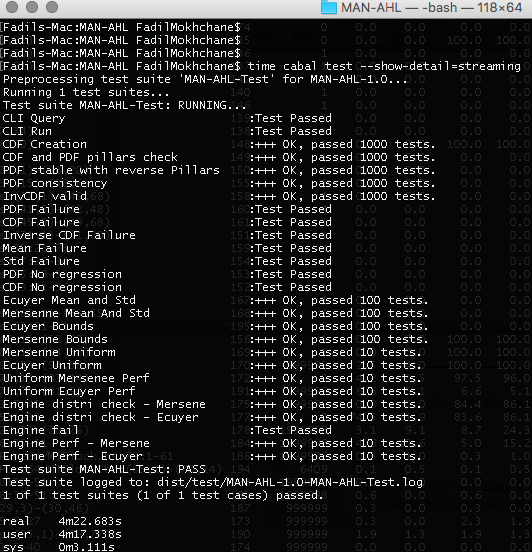
\includegraphics[width=0.7\textwidth]{img/tests.png}
\caption{Automated Testing}
\label{fig:tests}
\end{center}
\end{figure}

The following Test Suites, i.e. lists of tests, compose our test plan split by modules.
There is more on the testing in \autoref{sec:quality}. We expand on what is a correct 
metric for this problem.

\subsection{Test Data Sample}

The key test data sample used throughout the testing 
is the generation of PDF pillars.
We tried to pick a realistic sample :
The pillars can have 1 to 10 pillars. Their summed probability are always less 
than or equal to 1.  Each probability is within the $]0, 1]$ bound.

We felt that the number of pillars was meant to be small. It is unlikely
the software will be used with a million pillars. 

\subsection{Analytics Testing} 
These are the unit tests for the Analytics only.
\begin{description}
	\item [CDF creation]
		Given a 1000 pseudo random PDF, we ensure 
		that the last pillar of the CDF is 1.
		As the CDF is build incrementally, this gives a good sense that
		the CDF construction has been correct.
	\item [InverseCDF, CDF and PDF pillars check]
		Given a 1000 pseudo random PDF, we ensure that
		the pillars on the x axis of the PDF and CDF are the pillars on the y
		axis of the Inverse CDF.
	\item [PDF Stable]
		Given a 1000 pseudo random PDF pillars, 
		we ensure that we get the same PDF given the reverse input.
	\item [PDF consistency]
		Given a 1000 pseudo random PDF, 
		we ensure that the sum of the PDF pillars probabilities are 
		equal to 1. We indeed modelise the non selected element
		only in the CDF.
	\item [Inverse CDF valid]
		Given a 1000 pseudo random PDF,
		we build the CDF and we ensure that for a random number of
		x values within 0 and 1 we always recover a x pillars of the PDF.
	\item [PDF failure]
		We test the expecture failure of the PDF construction. 
		We can't have negative values. We need at least one valid pillar.
		The pillars with 0 probabilities are discarded.
		And the sum of the PDF pillars probabilities must be 
		equal to one.
	\item [Inverse CDF Failure]
		We check that the inverse CDF function raise an
		exception if the x input is outside the correct bounds, 
		$\left[0, 1\right]$.
	\item [Mean and Standard Deviation Failure]
		These functions raise an exception for empty lists.
		We test it automatically.
	\item [PDF and Inverse CDF Non Regression]
		We ensure without randomness that given a set of pillars,
		we recover the expected Inverse CDF and PDF.
	\item [Statistics Non Regression]
		We ensure without randomness that given a set of pillars,
		we recover the expected statistics used in the post processing
		of the Stats engines.
\end{description}
\subsection{Uniform Engine Testing} 

These are the unit tests for the bounded uniform pseudo random engine.
	
\begin{description}
	\item [Mean and Standard Deviation]
		Given a large number of random number generated for
		both Ecuyer and Mersenne, i.e. $100000$.
		We ensure that the mean and the standard deviation 
		of the distributions are still the same. Run 10 times.
		We ensure that the uniform random number engines keep
		the same properties.
	\item [Bounds]
		Test ensuring that the uniform pseudo random generators
		generate probabilities with the $[0, 1]$ bound.
		Run $10$ times for $1000000$ random numbers.
	\item [Uniform]
		Ensure that the ditributions generated are uniform,
		by making sure that we match a flat distribution at 0.001
		precision on the standard deviation of the difference
		between the PDFs.
		Run 10 times for $100000$ random numbers.
	\item [Performance]
		Ensure that the pseudo random numbers keep at
		least the same performance.
		Run 10 times for $100000$ random numbers.
	\item [Engine Fail]
		Ensure that the construction of the engine 
		handles all the expected failure.
\end{description}

\subsection{Weighted Engine Testing} 
These are the unit tests for the weighted pseudo random engine.
All tests are run using the two available uniform pseudo random
generators. 
These are like the integration tests as they use most of the library.
\begin{description}
	\item [Distribution check]
		We check that we recover the PDF distribution from
		a sample of 1000000 random numbers at $0.1\%$ precision
		on the standard deviation of the differences with the 
		generated PDF.
		We run this for 10 pseudo random PDF.
	\item [Engine Fail]
		Ensure that the construction of the engine 
		handles all the expected failure.
	\item [Performance]
		Ensure that the engine keep at least the same performance.
		Run 10 times for $100000$ random  numbers	
\end{description}	

\subsection{CLI Testing}
We test that the API produce what is expected.
\begin{description}
	\item [Query]
	We test that given an argument list, we produce the expected
	Query.
	\item[Run]
	We test that for given a Query, we produce the expected Result.
\end{description}

%-------------------------------------------------------------------------------
\section{Qualitative Analysis}
\label{sec:quality}
We realise that we maybe be beyond the scope of the initial
question, which was to implement a \emph{nextNum} function.
However how to test it efficiently ? It is a very hard question.
This led us to look at the distribution of the results to ensure
the quality of the numbers generated.

In this section, we will look at the number generated and try
to find the best parameters for this software.

\subsection{Metrics}
To assess the quality of a random number engine, we use
simple statistics. 

There are two keys elements that drive the results :
the input discrete probability function with $k$ pillars and
the output discrete probability function deducted from a
simulation of $n$ random numbers.

Hence we look at different input PDF with various $k$,
and the output PDF with various $n$. 
This data gives us intuitions about what are the right
parameters, $n$ and $k$ to use for our engines.

We also have two random numbers generators, 
Mersenne and Ecuyer, available. We compare them thoughout.

As our weighted probability engine depends on
the uniform probability engine, we test first the uniform engine.

The metrics we look at are:
\begin{itemize}
	\item the difference between the input and output pdf,
	\item the standard deviation of these differences,
	\item the mean of these differences, hopefully close to zero,
	\item and the highest and lowest differences.
\end{itemize}

\subsection{Uniform Distribution}

The input PDF for a uniform distribution is flat. The probabilities
should be the same for each bucket. 

\autoref{tab:uni.test} presents several runs for various number of random
numbers for each random number generators, which can be use in
the bounded uniform probability engine.
% Table generated by Excel2LaTeX from sheet 'Sheet5'
\begin{table}[htbp!]
  \centering \tiny
    \begin{tabular}{r|rrrrrr}
    \multicolumn{1}{r}{} & \multicolumn{2}{c}{1000000} & \multicolumn{2}{c}{100000} & \multicolumn{2}{c}{10000} \\
    \multicolumn{1}{r}{} & Mersenne & Ecuyer & Mersenne & Ecuyer & Mersenne & Ecuyer \\
\cmidrule{2-7}    Mean  & 5.55E-19 & 4.16E-19 & 4.86E-19 & 2.78E-19 & 5.55E-19 & 4.16E-19 \\
    StdDev  & 1.08E-04 & 1.27E-04 & 4.42E-04 & 4.80E-04 & 1.47E-03 & 1.29E-03 \\
    Highest  & 1.89E-04 & 2.89E-04 & 9.90E-04 & 1.01E-03 & 3.80E-03 & 2.50E-03 \\
    Lowest  & -2.91E-04 & -2.93E-04 & -1.56E-03 & -1.25E-03 & -3.10E-03 & -2.60E-03 \\
    \end{tabular}%
  \caption{Uniform Distribution Test}
  \label{tab:uni.test}%
\end{table}%

The best standard deviation we achieve is of the order of $e-4$.
The mean is very close to zero with both generators and the results 
are very similar.
Hence setting $n$ to 1000000 for more accurate testing, 
i.e. of the order of $e-4$, is recommanded.

We tried various $k$, less than 100 to remain realistic. It has no impact on the
results as expected.

\subsection{Weighted Distribution}

Therefore we can't expect to achieve better accuracy with the
weighted probability engine as it relies on the bounded uniform engine.

We present in \autoref{tab:w.test}, the result of multiple runs with various $n$.
% Table generated by Excel2LaTeX from sheet 'Sheet5'
\begin{table}[htbp!]
  \centering \tiny
    \begin{tabular}{r|rrrrrr}
    \multicolumn{1}{r}{} & \multicolumn{2}{c}{1000000} & \multicolumn{2}{c}{100000} & \multicolumn{2}{c}{10000} \\
    \multicolumn{1}{r}{} & Mersenne & Ecuyer & Mersenne & Ecuyer & Mersenne & Ecuyer \\
\cmidrule{2-7}    Mean  & -3.73E-18 & -3.36E-18 & -3.45E-18 & -3.96E-18 & -3.38E-18 & -3.26E-18 \\
    StdDev  & 1.71E-04 & 1.49E-04 & 5.14E-04 & 4.61E-04 & 1.79E-03 & 1.91E-03 \\
    Highest  & 7.88E-04 & 2.70E-04 & 1.13E-03 & 8.00E-04 & 5.20E-03 & 5.50E-03 \\
    Lowest  & -2.99E-04 & -3.61E-04 & -1.34E-03 & -1.25E-03 & -5.10E-03 & -5.52E-03 \\
    \end{tabular}%
  \caption{Weighted Distribution Test}
  \label{tab:w.test}%
\end{table}%
The result are very close to the precision of the uniform engine. 
We therefore recommand the same setting as before for $n$ and $k$.

%-------------------------------------------------------------------------------
\section{Performance Analysis}

\subsection{Complexity Analysis}
We commented some of the code with the complexities.
The computation of the weighted distribution for $n$ random number generated, 
i.e. the function \emph{allStats}, with a PDF of $k$ pillars, is :
\[
	O(n . log (k) . rng )
\]
where $rng$ is the complexity of the raw random number generator.

\subsection{Uniform Engine Performance}
\autoref{tab:uni.perf} presents the result of many runs with various $n$ and
the heap that was allocated during the run and the time taken.
\begin{table}[htbp!]
  \centering \tiny
    \begin{tabular}{r|rrrrrr}
    \multicolumn{1}{r}{} & \multicolumn{2}{c}{1000000} & \multicolumn{2}{c}{100000} & \multicolumn{2}{c}{10000} \\
    \multicolumn{1}{r}{} & Mersenne & Ecuyer & Mersenne & Ecuyer & Mersenne & Ecuyer \\
\cmidrule{2-7}    Heap  & 2,724,561,112 & 3,360,007,920 & 274,635,272 & 338,190,648 & 29,602,472 & 35,953,944 \\
    Time  & 3.576 & 3.707 & 0.347 & 0.373 & 0.041 & 0.041 \\
    \end{tabular}%
  \caption{Uniform Engine Performance}
  \label{tab:uni.perf}%
\end{table}%
Most of the heap allocation and the time is consumed by the underlying 
random number generator, the various engines adds only minor overhead, 
as shown on the profiling results, c.f. \autoref{fig:perf1} and \autoref{fig:perf2}.
We can see that the time and space are linear with respect to $n$. 
\begin{figure}[h!]
\begin{center}
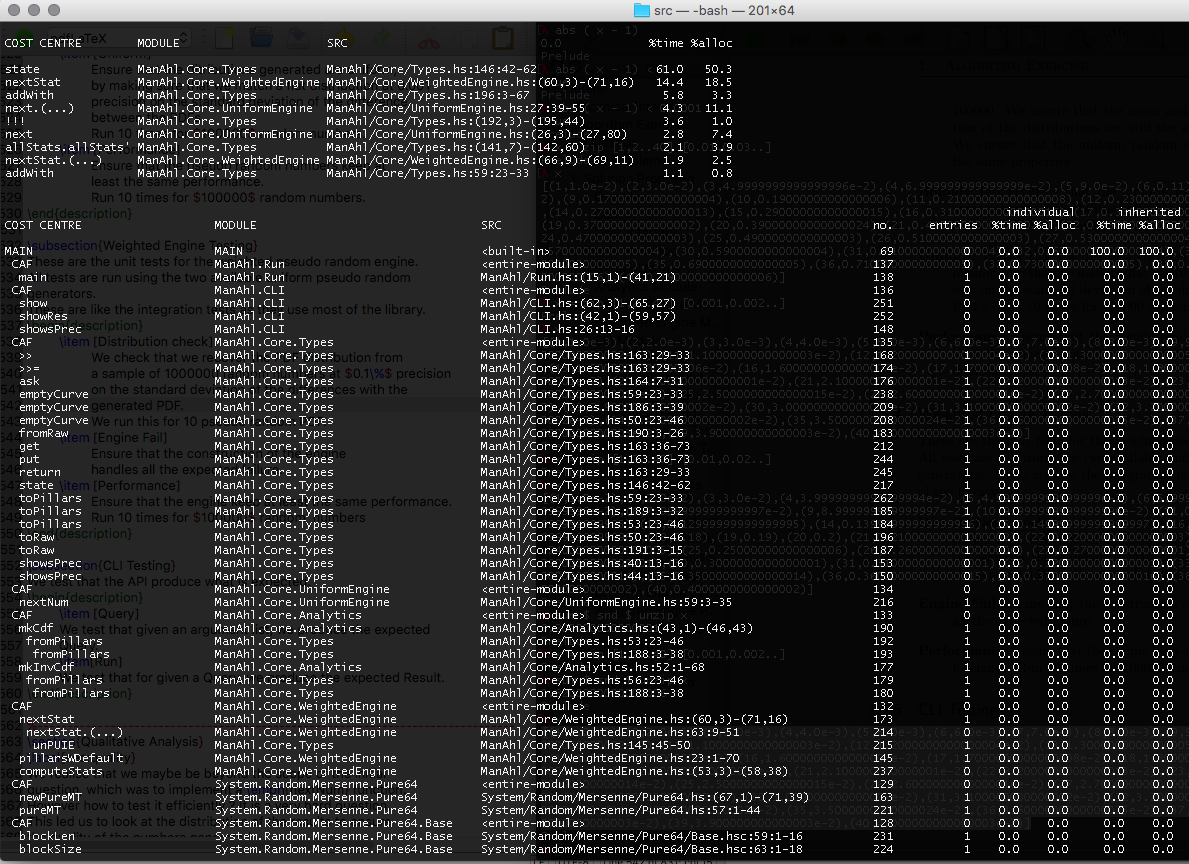
\includegraphics[width=1\textwidth]{img/prof1.png}
\caption{Performance Profiling 1}
\label{fig:perf1}
\end{center}
\end{figure}
\begin{figure}[h!]
\begin{center}
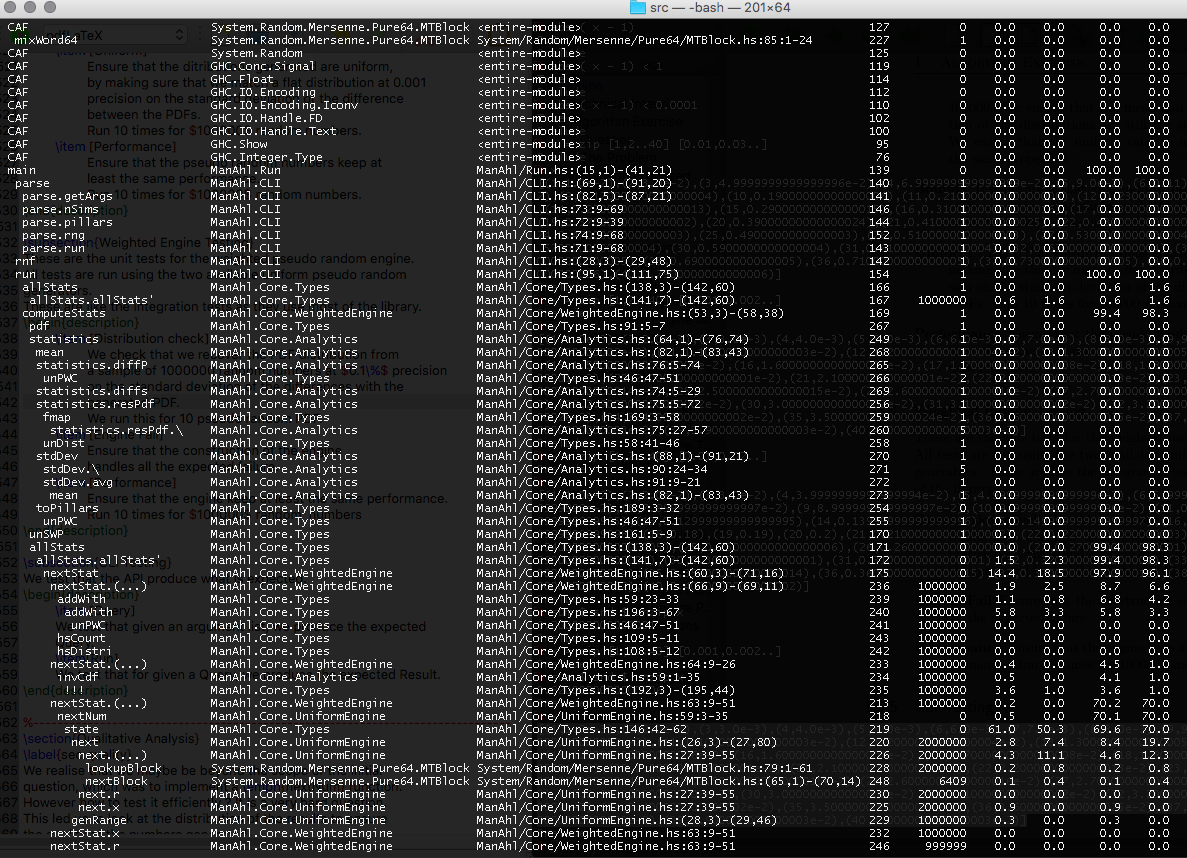
\includegraphics[width=1\textwidth]{img/prof2.png}
\caption{Performance Profiling 2}
\label{fig:perf2}
\end{center}
\end{figure}
%\begin{figure}[h!]
%\begin{center}
%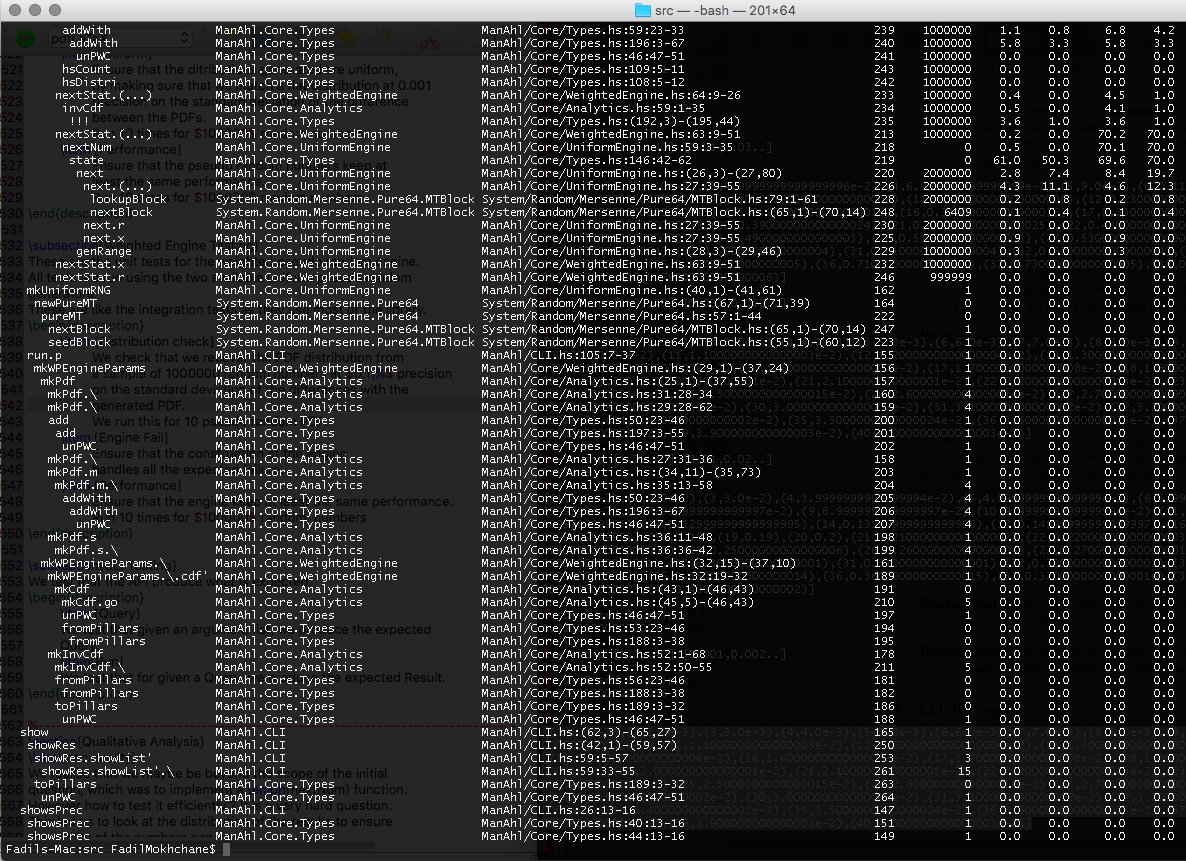
\includegraphics[width=1\textwidth]{img/prof3.png}
%\caption{Performance Profiling 3}
%\label{fig:perf3}
%\end{center}
%\end{figure}
We can conclude that the complexity of the inner random number generators
are $O(1)$ in time and $O(n)$ in space. Indeed the function \emph{allStats} for the
\emph{StatUniEngine} does not store the number generated, 
just the distribution of these.

We notice that Ecuyer take much more space, therefore our default setting
is set to Mersenne.

\subsection{Weighted Engine Performance}

\autoref{tab:w.perf} presents similar results for the \emph{StatWPEngine}, 
i.e. the statistic weighted probability engine.
\begin{table}[htbp!]
  \centering \tiny
    \begin{tabular}{r|rrrrrr}
    \multicolumn{1}{r}{} & \multicolumn{2}{c}{1000000} & \multicolumn{2}{c}{100000} & \multicolumn{2}{c}{10000} \\
    \multicolumn{1}{r}{} & Mersenne & Ecuyer & Mersenne & Ecuyer & Mersenne & Ecuyer \\
\cmidrule{2-7}    Heap  & 2,777,630,784 & 3,419,213,784 & 281,175,032 & 344,423,280 & 30,695,560 & 37,067,344 \\
    Time  & 3.612 & 3.81  & 0.357 & 0.379 & 0.038 & 0.043 \\
    \end{tabular}%
  \caption{Weighted Engine Performance}
  \label{tab:w.perf}%
\end{table}%
The results shows that there is little overhead for the weighted probabilities
engines. The results are very similar to \autoref{tab:uni.perf}.
This conforts us in the computation of our complexities.

%-------------------------------------------------------------------------------
\section{Possible Extensions}
Here is a list of possible extension we could add.
\begin{description}
	\item [Analytics]
	Further abstract the PDF, CDF, InvCDF to handle all kind of keys.
	
	Review the design of the statistics.
	\item [Testing]
	We could run the tests on different environments to ensure the portability of 
	the code.
	\item [UI] 
	A nice extension would be to add a Graphic User Interface,
	using the library 
	\href{https://hackage.haskell.org/package/threepenny-gui}{threepenny-gui}
	to create a portable Web application. 

	Also we could integrate a plot library to display the distribution of 
	random numbers.
\end{description}

%-------------------------------------------------------------------------------
\newpage
\chapter{SQL Exercise}
\section{Question}
Given the following tables
\begin{lstlisting}[
           language=SQL,
           showspaces=false,
           basicstyle=\ttfamily,
           numbers=left,
           numberstyle=\tiny,
           commentstyle=\color{gray}
        ]
CREATE TABLE Product
(
product_id number primary key,
name varchar2(128 byte) not null,
rrp number not null,
available_from date not null
);
CREATE TABLE Orders
(
order_id number primary key,
product_id number not null,
quantity number not null,
order_price number not null,
dispatch_date date not null,
foreign key (product_id) references Product(product_id)
);
\end{lstlisting}
Write an sql query to find books that have sold fewer than 10 copies in the last year, 
excluding books that have been available for less than 1 month.

Some example data, intended to give an idea of the sort of data that might exist, 
can be found below. Note that the data is not complete, 
nor does it necessarily cover all the cases that might be encountered.

\begin{center}
    \begin{tabular}{| l | l | l | l |}
    \hline
	product\_id & name & rrp & available\_from \\
	\hline 
	101 & Bayesian Methods for ...& 94.95 & (last thursday) \\
	102 & (next year) in Review (preorder) & 21.95 & (next year) \\
	103 & Learn Python in Ten Minutes & 2.15 & (three months ago) \\
	104 & sports almanac (1999-2049) & 3.38 & (2 years ago) \\
	105 & finance for dummies & 84.99 & (1 year ago)  \\
	\hline
    \end{tabular}
\end{center}
\begin{center}
    \begin{tabular}{| l | l | l | l | l |}
    \hline
	order\_id & product\_id & quantity & order\_price & dispatch\_date \\
	\hline 
	1000 & 101 & 1 & 90.00 & (two months ago) \\
	1001 & 103 & 1 & 1.15 & (40 days ago) \\
	1002 & 101 & 10 & 90.00 & (11 months ago) \\
	1003 & 104 & 11 & 3.38 & (6 months ago) \\
	1004 & 105 & 11 & 501.33 & (two years ago) \\
	\hline
    \end{tabular}
\end{center}

\section{Solution Proposed}
We can solve the problem by running a query like:
\begin{lstlisting}[
           language=SQL,
           showspaces=false,
           basicstyle=\ttfamily,
           numbers=left,
           numberstyle=\tiny,
           commentstyle=\color{gray}
        ]
SELECT p.name
FROM  (
   SELECT product_id, name FROM Product 
      WHERE available_from <=  (today - 1 month)
) p
LEFT OUTER JOIN (
   SELECT product_id, SUM(quantity) nb FROM Orders
      WHERE dispatch_date >= (today - 1 year)
      GROUP BY product_id
      HAVING nb < 10
) o
   ON p.product_id = o.product_id
\end{lstlisting}

Adding indexes to the columns on which we join and maybe query would improve 
the performance. 
A query plan of the execution would indicate what is the best design for this 
database scheme.


\end{document}
